\part{Problem}
\label{partProb}
Let $\Omega\subset\R^3$ be a bounded simply-connected domain with a
Lipschitz continuous boundary $\Gamma$. Let $\Gamma_0,\dots,\Gamma_I$
be the connected components of $\Gamma$.\\

We will use the following notations :
\begin{align*}
gradient(v)&=(\partial_x v, \partial_y v, \partial_z v)=\grad v\\
gradient(\mbf{v})&=\begin{pmatrix}
\partial_x v_x & \partial_y v_x & \partial_z v_x\\
\partial_x v_y & \partial_y v_y & \partial_z v_y\\
\partial_x v_z & \partial_y v_z & \partial_z v_z
\end{pmatrix}=\grad\mbf{v}\\
divergence(\mbf{v})&=\frac{\partial v_x}{\partial x}+\frac{\partial v_y}{\partial y}+\frac{\partial v_z}{\partial z}=\div \mbf{v}\\
curl(\mbf{v})&=\begin{pmatrix}
\partial_y v_z - \partial_z v_y\\
\partial_z v_x - \partial_x v_z\\
\partial_x v_y - \partial_y v_x
\end{pmatrix}=\curl \mbf{v}\\
curl(curl(\mbf{v}))&=\curll \mbf{v}\\
H^1(\Omega) &= \{v \in L^2(\Omega)\;|\; \grad v\in L^2(\Omega)\}\\
H^1_0(\Omega) &= \{v \in H^1(\Omega)\; |\; v\restr{\Gamma} = 0\}\\
H(\mathrm{div};\Omega) &= \{\mbf{v} \in [L^2(\Omega)]^3\; |\; \div\mbf{v} \in L^2(\Omega) \}\\
H(\mathrm{curl};\Omega) &= \{\mbf{v} \in [L^2(\Omega)]^3\; |\; \curl\mbf{v} \in L^2(\Omega) \}\\
L^2_\sigma(\Omega) &= \{\mbf{v} \in [L^2(\Omega)]^3\; |\; \div \mbf{v} = 0\text{ et }\mbf{v}\cdot \mbf{n}\restr{\Gamma} = 0 \}\\
D^1(\Omega) &= \{\mbf{v} \in [H^1(\Omega)]^3\cap L^2_\sigma(\Omega)\; |\; (\curl \mbf{v}\cdot \mbf{n})\restr{\Gamma} = 0  \}
\end{align*}

We are looking for $(\mbf{v},p)$, corresponding to the velocity and the pressure, solutions of the incompressible Navier-Stokes equations in $Q_T=\Omega\times[0,T]$, where $\Omega$ is an open set in $\R^3$ and $\partial\Omega$ its boundary, with initial condition and general impermeable boundary conditions.
\begin{pb}\label{start}
Find $(\mbf{v},p)$ such that :
\begin{equation*}
\left\{\begin{aligned}
&\frac{\partial \mbf{v}}{\partial t} + (\curl  \mbf{v})\times \mbf{v} + \grad q + \frac{1}{Re}\curll  \mbf{v}-\mbf{f} = 0\\
&\div \mbf{v} = 0\\
&\mbf{v}\big\rvert_{t=0} = \mbf{v}_0\\
&\mbf{v}\cdot \mbf{n}\restr{\Gamma} = \alpha_0\\
&(\curl  \mbf{v})\cdot \mbf{n}\restr{\Gamma} = \alpha_1\\
&(\curll  \mbf{v})\cdot \mbf{n}\restr{\Gamma} = \alpha_2
\end{aligned}\right.
\end{equation*}
where $q = \frac{|\mbf{v}|^2}{2}+p$.\\
\end{pb}
This problem has non standards boundary conditions. Rather than Dirichlet conditions, we use $\nabla^k\times\mbf{v}\cdot\mbf{n}\restr{\Gamma}$ for $k=0,1,2$ with $\nabla^0\times=Id$.\\
There have been few studies about these conditions and the industry rarely uses it. We can cite the works of V. Girault \cite{girault90-1}, H. Bellout, J. Neustuppa and P. Penel \cite{Penel2004}. The principle is a Galerkin type decomposition that can be related to the works of E. Deriaz and V. Perrier \cite{Deriaz2009249}.\\

The interest for Plastic Omnium is to be able to split the variables in time and space, and hence compute longer simulations. Furtermore, this could mean that we wouldn't need wall functions boundary condition, and so the boundary layer become needless.\\ 

We can now explain the resolution's strategy in the chapter \ref{strategy}, then study each step of the resolution in more details in \ref{fv}.

\chapter{Resolution's Strategy}
\label{strategy}
According to \cite{Penel2004}, the existence and unicity of the solution are guaranteed if the solution lives in $D^1$, which means that $\nabla^k\times\mbf{v}\cdot\mbf{n}\restr{\Gamma}=0$ for $k=0,1$. We need to relief these boundary conditions with a function $\mbf{a}$. We want to write $\mbf{v}=\mbf{u}+\mbf{a}$, such that :\\
\begin{equation}\label{v}
\begin{array}{c|ccccc}
& \mbf{v} & = & \mbf{a} & + & \mbf{u}\\ \hline
\div\star & 0 & & 0 & & 0\\ \hline
\star\cdot \mbf{n}\restr{\Gamma} & \alpha_0 & & \alpha_0 & & 0\\ \hline
\curl\star\cdot \mbf{n}\restr{\Gamma} & \alpha_1 & & \alpha_1 & & 0\\ \hline
\curll\star\cdot \mbf{n}\restr{\Gamma} & \alpha_2 & & \alpha_2 & & 0
\end{array}
\end{equation}
We have $\mbf{u}\in D^1(\Omega)$ to define the solution in the interior of the domain and $\mbf{a}\in [L^2(\Omega)]^3$ that we use for the boundary conditions.
\begin{pb}\label{a}
Find $\mbf{a}\in [L^2(\Omega)]^3$ such that :
\begin{equation*}
\left\{\begin{aligned}
&\mbf{a}=\grad a_0 + \curl\mbf{a}_1 + \mbf{a}_2\\
&\div \mbf{a} =0\\
&\mbf{a}\cdot \mbf{n}\restr{\Gamma} = \alpha_0\\
&(\curl \mbf{a})\cdot \mbf{n}\restr{\Gamma} = \alpha_1\\
&(\curll\mbf{a})\cdot\mbf{n}\restr{\Gamma} = \alpha_2
\end{aligned}\right.
\end{equation*}
\end{pb}
By applying the divergence and the boundary contions to the first lign, it leads to :
\begin{center}
\begin{tabular}{c|ccccccc}
& $\mbf{a}$ & = & $\grad a_0$ & + & $\curl \mbf{a}_1$ & + & $\mbf{a}_2$ \\ \hline
$\div\star$ & 0 & & $\laplace a_0$ & & 0 & & 0\\ \hline
$\star\cdot \mbf{n}\restr{\Gamma}$ & $\alpha_0$ & & $\alpha_0$ & & 0 & & 0\\ \hline
  $\curl\star\cdot \mbf{n}\restr{\Gamma}$ & $\alpha_1$ & & 0 & & $\alpha_1$ & & 0\\ \hline
  $\curll\star\cdot\mbf{n}\restr{\Gamma}$ & $\alpha_2$ & & 0 & & 0 & & $\alpha_2$
\end{tabular}
\end{center}
With the two first ligns of the table, we get the problem :
\begin{pb}\label{pba0}
Find $a_0$ such that :
\begin{equation*}
\left\{\begin{aligned}
&-\laplace a_0 = 0\\
&\grad a_0\cdot \mbf{n}\restr{\Gamma}=\alpha_0
\end{aligned}\right.
\end{equation*}\end{pb}
This problem allows us to find $a_0$ up to a constant, we need to use Lagrange multiplier to add a constraint, for example $\int_Omega a_0=0$. We can choose the constant because we only need the gradient.\\
We'll discuss which way we solve the problem \ref{pba0} further.\\

Let $\mbf{a}_1$ solution of the mixed problem :
\begin{pb}\label{pba1}
Find $(\mbf{a}_1,\psi^1)$ tel que :
\begin{equation*}
\left\{\begin{aligned}
&\curll \mbf{a}_1 = \grad\psi^1\\
&\div \mbf{a}_1 = 0\\
&\mbf{a}_1\cdot \mbf{n}\restr{\Gamma} = 0\\
&\curl \mbf{a}_1\cdot \mbf{n}\restr{\Gamma} = 0\\
&\grad\psi^1\cdot \mbf{n}\restr{\Gamma} = \alpha_1
\end{aligned}\right.
\end{equation*}\end{pb}

Let $\mbf{a}_2$ solution of the following problem :
\begin{pb}\label{pba2}
  Find $\mbf{a}_2$ such that :
  \begin{equation*}
    \left\{\begin{aligned}
    &\curll\mbf{a}_2 = \bm{\epsilon}\\
    &\div \mbf{a}_2 = 0\\
    &\mbf{a}_2\cdot\mbf{n}\restr{\Gamma} = 0\\
    &\curl\mbf{a}_2\cdot\mbf{n}\restr{\Gamma} = 0\\
    &\curll\mbf{a}_2\cdot\mbf{n}\restr{\Gamma} = \alpha_2
    \end{aligned}\right.
  \end{equation*}
  Such that $\bm{\epsilon}\cdot\mbf{n} = \alpha_2$
\end{pb}

Once we know $\grad a_0$, $\curl\mbf{a}_1$ and $\mbf{a}_2$, we have $\mbf{a}$.\\

We can replace $\mbf{v}$ by $\mbf{u}+\mbf{a}$ in problem \ref{start} :
\[ \frac{\partial(\mbf{u}+\mbf{a})}{\partial t}+(\curl(\mbf{u}+\mbf{a}))\times(\mbf{u}+\mbf{a}) + \grad (\frac{|\mbf{u}+\mbf{a}|^2}{2}+p) + \frac{1}{Re}\curll(\mbf{u}+\mbf{a}) - \mbf{f} = 0 \]
Which leads to, by noting $\pi_a=\frac{|\mbf{u}+\mbf{a}|^2}{2}+p$ :
\[ \frac{\partial \mbf{u}}{\partial t}+\frac{\partial \mbf{a}}{\partial t} + (\curl \mbf{u}+\curl \mbf{a})\times(\mbf{u}+\mbf{a}) + \grad\pi_{\mbf{a}} + \frac{1}{Re}(\curll \mbf{u}+\curll \mbf{a}) - \mbf{f} = 0 \]
We have that $\curll \mbf{a} = \bm{\epsilon}$, then if $\mbf{f_a}=\mbf{f}-\frac{\partial \mbf{a}}{\partial t} - (\curl \mbf{a})\times \mbf{a} - \bm{\epsilon}$, we have the following problem :
\begin{pb}\label{pbu}
Find $\mbf{u}$ such that :
\begin{equation*}
\left\{\begin{aligned}
&\frac{\partial \mbf{u}}{\partial t} + (\curl \mbf{u})\times \mbf{u} + (\curl \mbf{u})\times \mbf{a} +(\curl \mbf{a})\times \mbf{u} + \grad \pi_{\mbf{a}} +\frac{1}{Re}\curll  \mbf{u} - \mbf{f_a} = 0\\
&\div \mbf{u} = 0\\
&\mbf{u}\big\rvert_{t=0} = \mbf{v}_0 - \mbf{a}(0,\cdot)\\
&\mbf{u}\cdot \mbf{n}\restr{\Gamma} = 0\\
&(\curl \mbf{u})\cdot \mbf{n}\restr{\Gamma} = 0\\
&(\curll  \mbf{u})\cdot \mbf{n}\restr{\Gamma} = 0
\end{aligned}\right.
\end{equation*}\end{pb}

Using a Galerkin decomposition, we have :
\begin{equation}\label{u}
\mbf{u}(t,\cdot) = \sum_{i=1}^{\infty} c_i(t)\mbf{g}_i(\cdot)
\end{equation}
where we have separeted the variables depending on time and space. The coefficients $c_i$ include all informations depending on the time, whereas the functions $\mbf{g}_i$ carry the spacial component.\\

Since $\mbf{u}\in D^1(\Omega)=D(\mathrm{rot}_{imperm})$, according to \cite{Penel2004}, a basis of this space is the eigen functions $\mbf{g}_i$ of the curl operator.
So, we want to solve the eigen problem :
\begin{pb}\label{pbcurl}
Find $(\lambda_i,\mbf{g}_i)\in\R\times D^1(\Omega)$ such that :
\begin{equation*}
\left\{\begin{aligned}
&\curl  \mbf{g}_i = \lambda_i \mbf{g}_i\\
&\div\mbf{g}_i = 0\\
&\mbf{g}_i\cdot \mbf{n}\restr{\Gamma} = 0\\
&\curl \mbf{g}_i\cdot \mbf{n}\restr{\Gamma} = 0
\end{aligned}\right.
\end{equation*}\end{pb}

By injecting \ref{u} in the problem \ref{pbu}, we get :
\begin{align*}
\frac{\partial}{\partial t}\left(\sum_{i=1}^\infty c_i\mbf{g}_i\right) &+ \left(\curl \left(\sum_{i=1}^\infty c_i\mbf{g}_i\right)\right)\times \left(\sum_{i=1}^\infty c_i\mbf{g}_i\right) + \left(\curl \left(\sum_{i=1}^\infty c_i\mbf{g}_i\right)\right)\times \mbf{a}&\\
&+ (\curl \mbf{a})\times \left(\sum_{i=1}^\infty c_i\mbf{g}_i\right) + \grad \pi_{\mbf{a}} +\frac{1}{Re}\curll  \left(\sum_{i=1}^\infty c_i\mbf{g}_i\right) - \mbf{f_a} =0\\
\end{align*}

Using the linearity of the derivative operator, as well as that of the curl operator, we have :
\begin{pb}\label{pbc}
Find $(c_i)$ such that :
\begin{align*}
\sum_{i=1}^\infty\frac{\partial c_i}{\partial t}\mbf{g}_i &+ \sum_{i=1}^\infty\sum_{j=1}^\infty c_i c_j((\curl\mbf{g}_i)\times \mbf{g}_j) + \sum_{i=1}^\infty c_i((\curl\mbf{g}_i)\times \mbf{a})\\
& + \sum_{i=1}^\infty c_i((\curl\mbf{a})\times \mbf{g}_i) + \grad \pi_{\mbf{a}} +\frac{1}{Re}\sum_{i=1}^\infty c_i\curll\mbf{g}_i - \mbf{f_a} = 0\\
\end{align*}
with \[ \sum_{i=1}^\infty c_i(0)\mbf{g}_i = \mbf{v_0}-\mbf{a}(0,\cdot) \]
\end{pb}

To summarize, we have to :
\begin{enumerate}
\item generate the basis $\{\mbf{g}_i\}$ from the eigen functions of the curl operator by solving \ref{pbcurl} as explain in the chapter \ref{eigen}.
\item find $\mbf{a}$ to decompose $\mbf{v}$ as $\mbf{u}+\mbf{a}$, for this, we solve the problems \ref{pba0},\ref{pba1} and \ref{pba2}. Which allows us to compute $\mbf{a}$ with \ref{a}. This part is details in \ref{relev}.
\item solve problem \ref{pbc} to find the coefficients $c_i$. This is explain in chapter \ref{spectre}.
\item recompose $\mbf{v}=\mbf{u}+\mbf{a}$, and find $p$ to get the solution of the problem \ref{start}. The chapter \ref{pressure} explains how to do it.
\end{enumerate}

The strategy is presented in the figure \ref{org1}.
\begin{figure}[H]
  \centering
  \begin{tikzpicture}
    \node[draw,scale=\taille,fill=green!50] (alpha0) at (-1,10) {$\alpha_0$};
    \node[draw,scale=\taille,fill=gray!50,label={[xshift=0.9cm]\ref{pba0}}] (pba0) at (-1,8){
      $\begin{aligned}
        -\laplace a_0&=0\\
        \grad a_0\cdot \mbf{n} &= \alpha_0
      \end{aligned}$
    };
    \node[draw,scale=\taille,fill=blue!50] (grada0) at (-1,5.5) {$\grad a_0$} ;
    \node[draw,scale=\taille,fill=green!50] (alpha1) at (1.5,10) {$\alpha_1$};
    \node[draw,scale=\taille,fill=gray!50,label={[xshift=1.1cm]\ref{pba1}}] (pba1) at (1.5,8){
      $\begin{aligned}
        \curll \mbf{a}_1 = \grad\psi^1\\
        \div \mbf{a}_1 = 0\\
        \mbf{a}_1\cdot \mbf{n}\restr{\Gamma} = 0\\
        \curl \mbf{a}_1\cdot \mbf{n}\restr{\Gamma} = 0\\
        \grad\psi^1\cdot \mbf{n}\restr{\Gamma} = \alpha_1
      \end{aligned}$
    } ;
    \node[draw,scale=\taille,fill=blue!50] (curla1) at (1.5,5.5) {$(\curl\mbf{a}_1,\grad\psi^1)$} ;
    \node[draw,scale=\taille,fill=green!50] (alpha2) at (4,10) {$\alpha_2$};
    \node[draw,scale=\taille,fill=gray!50,label={[xshift=1.1cm]\ref{pba2}}] (pba2) at (4,8){
      $\begin{aligned}
        \curll \mbf{a}_2 = \bm{\epsilon}\\
        \div \mbf{a}_2 = 0\\
        \mbf{a}_2\cdot \mbf{n}\restr{\Gamma} = 0\\
        \curl \mbf{a}_2\cdot \mbf{n}\restr{\Gamma} = 0\\
        \bm{\epsilon}\cdot \mbf{n}\restr{\Gamma} = \alpha_2
      \end{aligned}$
    } ;
    \node[draw,scale=\taille,fill=blue!50] (a2) at (4,5.5) {$(\curl\mbf{a}_2,\bm{\epsilon})$} ;
    \node[draw,scale=\taille,fill=gray!50,label={[xshift=1.5cm]\ref{a}}] (pba) at (1.5,4) {$\mbf{a}=\grad a_0+\curl\mbf{a}_1+\mbf{a}_2$};
    \node[draw,scale=\taillem,fill=blue!50] (a) at (1.5,3) {$\mbf{a}$} ;
    \node[draw,scale=\taille,fill=gray!50,label={[xshift=1.1cm]\ref{pbcurl}}] (pbcurl) at (10,8) {
      $\begin{aligned}
        \curl \mbf{g}_i = \lambda_i\mbf{g}_i\\
        \div\mbf{g}_i = 0\\
        \mbf{g}_i\cdot \mbf{n}\restr{\Gamma} = 0\\
        \curl\mbf{g}_i\cdot \mbf{n}\restr{\Gamma} = 0
      \end{aligned}$
    } ;
    \node[draw,scale=\taille,fill=yellow!50] (lambdagi) at (10, 5.5) {$(\lambda_i,\mbf{g}_i)$} ;
    \node[draw,scale=\taille,fill=green!50] (f) at (6.75,5.5) {$\mbf{f}$};
    \node[draw,scale=\taille,fill=green!50] (c0) at (7.75,5.5) {$c_i(0)$};
    \node[draw,scale=\taille,fill=gray!50,label={[xshift=4.5cm]\ref{pbc}}] (pbc) at (8.5,3) {
      $\begin{aligned}
        \sum_{i=1}^\infty\frac{\partial c_i}{\partial t}\mbf{g}_i &+ \sum_{i=1}^\infty\sum_{j=1}^\infty c_i c_j((\curl\mbf{g}_i)\times \mbf{g}_j) + \sum_{i=1}^\infty c_i((\curl\mbf{g}_i)\times \mbf{a})\\
        & + \sum_{i=1}^\infty c_i((\curl\mbf{a})\times \mbf{g}_i) + \grad \pi_{\mbf{a}} +\frac{1}{Re}\sum_{i=1}^\infty c_i\curll\mbf{g}_i - \mbf{f_a} = 0
      \end{aligned}$
    };
    \node[draw,scale=\taillem,fill=blue!50] (u) at (8.5,1) {$\mbf{u}$} ;
    \node[draw,scale=\taille,fill=gray!50] (pbv) at (5,-0.5) {$\mbf{v}=\mbf{a}+\mbf{u}$} ;
    \node[draw,scale=\tailleg,fill=red!50] (v) at (5,-2) {$(\mbf{v},p)$} ;

    \draw[->,>=latex] (alpha0) -- (pba0); \draw[->,>=latex] (pba0) -- (grada0); \draw[->,>=latex] (alpha1) -- (pba1); \draw[->,>=latex] (pba1) -- (curla1); \draw[->,>=latex] (alpha2) -- (pba2); \draw[->,>=latex] (pba2) -- (a2); \draw[->,>=latex] (grada0) -- (pba); \draw[->,>=latex] (curla1) -- (pba); \draw[->,>=latex] (a2) -- (pba); \draw[->,>=latex] (pba) -- (a); \draw[->,>=latex] (pbcurl) -- (lambdagi); \draw[->,>=latex] (a) -- (pbc); \draw[->,>=latex] (f) -- (pbc); \draw[->,>=latex] (c0) -- (pbc); \draw[->,>=latex] (lambdagi) -- (pbc); \draw[->,>=latex] (pbc) -- (u); \draw[->,>=latex] (u) -- (pbv); \draw[->,>=latex] (a) -- (pbv); \draw[->,>=latex] (pbv) -- (v);
  \end{tikzpicture}
  \caption{Flow chart of the resolution's strategy}\label{org1}
\end{figure}

\chapter{Weak Formulations}
\label{fv}
Now that how we proceed to solve the problem \ref{start} is clear, we can detail each step mentionned before.

\chapter{Problème aux valeurs propres}
On peut maintenant implémenter le problème aux valeurs propres du chapitre \ref{eigen} afin de trouver les couples $(\lambda_i,\mathbf{g_i})$ tel que $\rot\mathbf{g_i}=\lambda_i\mathbf{g_i}$ pour $i=1,\dots,M$. Les fonctions propres seront la base sur laquelle on va projeter $\mathbf{u}$ pour la décomposition de Galerkin \[ \mathbf{u}=\sum_{i=1}^M c_i\mathbf{g_i} \]
Comme les fonctions propres vivent dans $D^1$, un espace à divergence nulle, l'opérateur rotationnel et le laplacien sont identiques. Cependant, comme les fonctions tests implémentées dans Feel++ ne sont pas à divergence nulle, si on utilise le laplacien, il est nécessaire de rajouter une étape de tri pour avoir des fonctions à divergence nulle. Comme cela est très coûteux en temps de calcul, il vaut mieux utiliser directement l'opérateur rotationnel.

\section{Utilisation des éléments de Nedelec}
\subsection{Formulation variationnelle}
Ici, on veut s'appuyer sur les travaux de V. Girault \cite{girault90-1}. Pour cela, on a besoin de définir l'espace \[X = \{\mathbf{v}\in H(\mathrm{rot})\ |\ (\rot\mathbf{v}\cdot\mathbf{n})\restr=0 \}\]
On rappel les définitions suivantes :
\begin{align*}
L^2_\sigma(\Omega) &= \{\mathbf{v} \in [L^2(\Omega)]^3\ |\ \div \mathbf{v} = 0\text{ et }\mathbf{v}\cdot \mathbf{n}\restr = 0 \}\\
D^1(\Omega) &= \{\mathbf{v} \in [H^1(\Omega)]^3\cap L^2_\sigma(\Omega)\ |\ (\rot \mathbf{v}\cdot \mathbf{n})\restr = 0  \}
\end{align*}
De plus, on a (voir \cite{Girault79}) :
\[ [H^1(\Omega)]^3=H(\mathrm{rot})\cap H(\mathrm{div}) \]
D'où:
\begin{align*}
D^1(\Omega) &= \{\mathbf{v}\in [H^1(\Omega)]^3\cap L^2_\sigma(\Omega)\ |\ (\rot \mathbf{v}\cdot \mathbf{n})\restr = 0  \}&\\
&=\{\mathbf{v}\in H(\mathrm{rot})\cap H(\mathrm{div})\cap L^2_\sigma(\Omega)\ |\ (\rot \mathbf{v}\cdot \mathbf{n})\restr = 0  \}&\\
&&\text{ or }L^2_\sigma\subset H(\mathrm{div})\\
&=\{\mathbf{v}\in H(\mathrm{rot})\cap L^2_\sigma(\Omega)\ |\ (\rot \mathbf{v}\cdot \mathbf{n})\restr = 0  \}&\\
&=\{\mathbf{v}\in H(\mathrm{rot})\ |\ (\rot \mathbf{v}\cdot \mathbf{n})\restr = 0  \}\cap L^2_\sigma(\Omega)&\\
&=X\cap L^2_\sigma(\Omega)&
\end{align*}

Le problème aux valeurs propres \ref{curlcurl} est donc :\\
Trouver $(\mathbf{g},\lambda)\in X\cap L^2_\sigma\times\R$ tel que :
\begin{align}
\rott\mathbf{g}&=\lambda^2\mathbf{g} \label{impPb1}\\
\div\mathbf{g}&=0 \label{impPb2}\\
(\mathbf{g}\cdot\mathbf{n})\restr&=0 \label{impPb3}\\
(\rot\mathbf{g}\cdot\mathbf{n})\restr&=0 \label{impPb4}\\
(\rott\mathbf{g}\cdot\mathbf{n})\restr&=0 \label{impPb5}
\end{align}
Les conditions (\ref{impPb2}-\ref{impPb3}) sont satisfaites par le fait que $\mathbf{g}\in L^2_\sigma$ et la condition (\ref{impPb4}) par l'appartenance à $X$.\\

En passant à la forme variationnelle, et en suivant les mêmes étapes que dans le chapitre \ref{eigen}, on impose la condition (\ref{impPb5}) :
\[ \int_\Omega (\rot\mathbf{g})\cdot(\rot\bm{\varphi}) + \int_{\partial\Omega} \phi(\underbrace{(\rott \mathbf{g})\cdot\mathbf{n}}_{=0})= \lambda^2\int_\Omega \mathbf{g}\cdot\bm{\varphi} \]
On a donc le problème suivant :\\
Trouver $(\mathbf{g},\lambda)\in X\cap L^2_\sigma\times\R$ tel que $\forall \bm{\varphi}\in X\cap L^2_\sigma$ :
\[ \int_\Omega (\rot\mathbf{g})\cdot(\rot\bm{\varphi}) = \lambda^2\int_\Omega \mathbf{g}\cdot\bm{\varphi} \]

Ne pouvant pas utiliser directement des fonctions de bases à divergence nulle pour les éléments finis, on impose cette condition par un terme de pression fictif. On a donc :\\
Trouver $((\mathbf{g},p),\lambda)\in X\cap L^2_\sigma \times H^1 \times \R$ tel que $\forall (\bm{\varphi},q)\in X\cap L^2_\sigma \times H^1$ :
\begin{align*}
\int_\Omega (\rot\mathbf{g})\cdot(\rot\bm{\varphi}) + \int_\Omega\bm{\varphi}\grad p &= \lambda^2\int_\Omega \mathbf{g}\cdot\bm{\varphi}\\
\int_\Omega (\div\mathbf{g}) q &= 0
\end{align*}
En intégrant par partie la seconde équation, on obtient
\[ \int_\Omega (\div\mathbf{g}) q = \int_\Omega \mathbf{g}\grad q - \int_{\partial\Omega} (\underbrace{\mathbf{g}\cdot \mathbf{n}}_{=0})q = 0 \]
On peut donc imposer les contraintes (\ref{impPb2}-\ref{impPb3}), liées à $L^2_\sigma$, dans la formulation faible suivante :\\
Trouver $((\mathbf{g},p),\lambda)\in X \times H^1 \times \R$ tel que $\forall (\bm{\varphi},q)\in X \times H^1$ :
\[ \int_\Omega (\rot\mathbf{g})\cdot(\rot\bm{\varphi}) + \int_\Omega\bm{\varphi}\grad p + \int_\Omega \mathbf{g}\grad q = \lambda^2\int_\Omega \mathbf{g}\cdot\bm{\varphi} \]

Pour imposer la condition (\ref{impPb4}), on utilise une méthode de pénalisation, le problème \ref{curlcurl} devient donc :
\begin{pb}\label{pbeigenrot}
Trouver $((\mathbf{g},p),\lambda)\in H(\mathrm{rot}) \times H^1 \times \R$ tel que $\forall (\bm{\varphi},q)\in H(\mathrm{rot}) \times H^1$ :
\begin{equation*}
\int_\Omega (\rot\mathbf{g})\cdot(\rot\bm{\varphi}) + \int_\Omega\bm{\varphi}\grad p + \int_\Omega \mathbf{g}\grad q + \gamma\int_{\partial\Omega}(\rot\mathbf{g}\cdot\mathbf{n})(\rot\bm{\varphi}\cdot\mathbf{n}) = \lambda^2\int_\Omega \mathbf{g}\cdot\bm{\varphi}
\end{equation*}
avec $\gamma$ une très grande valeur.
\end{pb}

\subsection{Discrétisation}
Ainsi, la solution se trouvant dans $H(\mathrm{rot})$, la meilleure méthode serait d'utiliser des éléments conformes à cet espace, à savoir les éléments de Nedelec. Cela permettrait d'avoir $\rot\mathbf{g_i}\in [L^2(\Omega)]^3$. On gagnerait ainsi en régularité sur les fonctions propres.\\

En utilisant le même maillage que dans \ref{discGradh1}, on discrétise le problème en utilisant des éléments finis conformes au rotationnel, de degré $k$, nommés éléments de Nedelec (\cite{Nedelec80,Nedelec86}) et notés $\mathbb{N}_k$. Ceci nous permet d'introduire le sous-espace de $H(\mathrm{rot})$ suivant :
\[ N^k_h = \{ \mathbf{v}_h \in H(\mathrm{rot}) \; |\; \mathbf{v}_h{}_{|_K} \in \mathbb{N}_k\; \forall\; K \in \mathcal{T}_h\}\]

Le problème \ref{pbeigenrot} est donc approché par le problème discret :
\begin{pb}
Trouver $((\mathbf{g}_h,p_h),\lambda)\in N^0_h\times P_{c,h}^1 \times \R$ tel que $\forall  (\bm{\varphi}_h,q_h)\in N^0_h\times P_{c,h}^1$ :
\begin{equation*}
\int_\Omega (\rot\mathbf{g}_h)\cdot(\rot\bm{\varphi}_h) + \int_\Omega\bm{\varphi}_h\grad p_h + \int_\Omega \mathbf{g}_h\grad q_h + \gamma\int_{\partial\Omega}(\rot\mathbf{g}_h\cdot\mathbf{n})(\rot\bm{\varphi}_h\cdot\mathbf{n}) = \lambda^2\int_\Omega \mathbf{g}_h\cdot\bm{\varphi}_h
\end{equation*}
avec $\gamma$ une très grande valeur.
\end{pb}

\section{Utilisation des éléments de Lagrange}
\subsection{Formulation variationnelle}
Cependant, les éléments de Nedelec n'étant pas prêt dans Feel++, on se place dans un espace plus large, $H^1$, et on utilise des éléments de Lagrange. Cela implique que $\rot\mathbf{g}$ n'appartient pas forcément à $L^2$. Cette méthode est donc moins précise et elle introduit de nouvelles erreurs de calcul.\\

Ces erreurs mènent à une divergence non nulle, en reprenant l'équation du problème \ref{pbeigenrot}, on ajoute un terme de pénalisation en plus afin de forcer la divergence. On résout donc le système suivant :
\[ \int_\Omega (\rot\mathbf{g})\cdot(\rot\bm{\varphi}) + \int_\Omega\bm{\varphi}\grad p + \int_\Omega \mathbf{g}\grad q + \gamma\int_{\partial\Omega}(\rot\mathbf{g}\cdot\mathbf{n})(\rot\bm{\varphi}\cdot\mathbf{n}) + \alpha\int_\Omega \div\mathbf{g}\div\bm{\varphi} = \lambda^2\int_\Omega \mathbf{g}\cdot\bm{\varphi} \]

Cependant, on a toujours la condition $\mathbf{g}\cdot\mathbf{n}$ qui n'est pas respecter. On ajoute donc un troisième terme de pénalisation et on résout le problème :
\begin{pb}\label{pbeigenh1}
Trouver $((\mathbf{g},p),\lambda)\in [H^1(\Omega)]^3\times H^1 \times \R$ tel que $\forall (\bm{\varphi},q)\in [H^1(\Omega)]^3\times H^1$ :
\begin{align*}
\int_\Omega (\rot\mathbf{g})\cdot(\rot\bm{\varphi}) &+ \int_\Omega\bm{\varphi}\grad p + \int_\Omega \mathbf{g}\grad q & \\
&+ \gamma\int_{\partial\Omega}(\rot\mathbf{g}\cdot\mathbf{n})(\rot\bm{\varphi}\cdot\mathbf{n}) & (\ref{impPb4})\\
& + \alpha\int_\Omega \div\mathbf{g}\div\bm{\varphi} & (\ref{impPb2})\\
&+ \beta\int_{\partial\Omega}(\mathbf{g}\cdot\mathbf{n})(\bm{\varphi}\cdot\mathbf{n})  = \lambda^2\int_\Omega \mathbf{g}\cdot\bm{\varphi} & (\ref{impPb3})
\end{align*} \end{pb}

\subsection{Discrétisation}
Toujours avec le même maillage, on réutilise l'espace $P^k_{c,h}$ introduit dans \ref{discGradh1}. On utilise des éléments d'ordre 2 pour les $\mathbf{g}$ et d'ordre 1 pour $p$. Ce qui donne le problème discret suivant :
\begin{pb}\label{disceigenh1}
Trouver $((\mathbf{g}_h,p_h),\lambda)\in [P^2_{c,h}]^3\times P^1_{c,h} \times \R$ tel que $\forall (\bm{\varphi}_h,q_h)\in [P^2_{c,h}]^3\times P^1_{c,h}$ :
\begin{align*}
\int_\Omega (\rot\mathbf{g}_h)\cdot(\rot\bm{\varphi}_h) &+ \int_\Omega\bm{\varphi}_h\grad p_h + \int_\Omega \mathbf{g}_h\grad q_h \\
&+ \gamma\int_{\partial\Omega}(\rot\mathbf{g}_h\cdot\mathbf{n})(\rot\bm{\varphi}_h\cdot\mathbf{n})\\
& + \alpha\int_\Omega \div\mathbf{g}_h\div\bm{\varphi}_h \\
&+ \beta\int_{\partial\Omega}(\mathbf{g}_h\cdot\mathbf{n})(\bm{\varphi}_h\cdot\mathbf{n})  = \lambda^2\int_\Omega \mathbf{g}_h\cdot\bm{\varphi}_h
\end{align*} \end{pb}

En notant :
\begin{itemize}
\item $N_{h1}$ la dimension de $P^1_{c,h}$,
\item $\{\phi^1_i\}_{i=1,\dots,N_{h1}}$ une base de $P^1_{c,h}$,
\item pour tout $P^1_{c,h}\ni p_h=\sum_{i=1}^{N_{h1}} p_i\phi^1_i$, $P=(p_1,\dots,p_{N_{h1}})^T$,
\item $N_{h2}$ la dimension de $[P^2_{c,h}]^3$,
\item $\{\bm{\phi^2}_i\}_{i=1,\dots,N_{h2}}$ une base de $[P^2_{c,h}]^3$,
\item pour tout $[P^2_{c,h}]^3\ni \mathbf{u}_h=\sum_{i=1}^{N_{h2}} u_i\bm{\phi^2}_i$, $U=(u_1,\dots,u_{N_{h2}})^T$,
\item $a$ une forme bilinéaire de $[P^2_{c,h}]^3\times [P^2_{c,h}]^3$ tel que : 
\[ a(\mathbf{u},\mathbf{v})=\int_\Omega \rot \mathbf{u}\cdot \rot \mathbf{v} + \alpha\int_\Omega \div\mathbf{u}\div\mathbf{v} + \beta\int_{\partial\Omega}(\mathbf{u}\cdot\mathbf{n})(\mathbf{v}\cdot\mathbf{n}) + \gamma\int_{\partial\Omega}(\rot\mathbf{u}\cdot\mathbf{n})(\rot\mathbf{v}\cdot\mathbf{n}) \]
\item $b$ une forme bilinéaire de $[P^2_{c,h}]^3\times P^1_{c,h}$ tel que : \[ b(\mathbf{u},p) = \int_\Omega \mathbf{u}\cdot\grad p \]
\item $m$ une forme bilinéaire de $[P^2_{c,h}]^3\times [P^2_{c,h}]^3$ tel que : \[ m(\mathbf{u},\mathbf{v})=\int_\Omega \mathbf{u}\cdot\mathbf{v} \]
\end{itemize}

Alors la forme matricielle du problème \ref{disceigenh1} est :
\[ \begin{pmatrix} \tilde{A} & B^T\\ B & 0\end{pmatrix}\begin{pmatrix}U\\ P\end{pmatrix} = \lambda\begin{pmatrix} \tilde{M} & 0\\0 & 0 \end{pmatrix}\begin{pmatrix}U\\ P\end{pmatrix} \]
soit le problème aux valeurs propres hermitien généralisé :
\[ A X = \lambda M X \]
avec 
\begin{itemize}
\item $\tilde{A}\in M(\R)^{N_{h2}\times N_{h2}}$ et $\tilde{A}_{ij} = a(\bm{\phi^2}_i,\bm{\phi^2}_j)$,
\item $B\in M(\R)^{N_{h2}\times N_{h1}}$ et $B_{ij}=b(\bm{\phi^2}_i,\phi^1_j)$,
\item $\tilde{M}=M(\R)^{N_{h2}\times N_{h2}}$ et $\tilde{M}=m(\bm{\phi^2}_i,\bm{\phi^2}_j)$,
\item $A\in M(\R)^{(N_{h2}+N_{h1})\times(N_{h2}+N_{h1})}$ et $A=\begin{pmatrix} \tilde{A} & B^T\\ B & 0\end{pmatrix}$,
\item $M\in M(\R)^{(N_{h2}+N_{h1})\times(N_{h2}+N_{h1})}$ et $M=\begin{pmatrix} \tilde{M} & 0\\0 & 0 \end{pmatrix}$,
\item $X\in \R^{N_{h2}+N_{h1})}$ et $X=\begin{pmatrix}U\\ P\end{pmatrix}$.
\end{itemize}


\subsection{Implémentation}

Comme on cherche les solutions dans $[P^2_{c,h}]^3$, on utilise des éléments de Lagrange et non de Nedelec pour approcher les $\mathbf{g_i}$. Pour le terme de pression fictif, on utilise aussi des éléments de Lagrange, scalaire et d'ordre 1.\\ 
\lstinputlisting[linerange=space]{../../src/eigenprob.hpp}
Pour résoudre le problème $AX=\lambda MX$, on initialise $M$ comme une matrice de masse. On utilise pour cela une forme bilinéaire :\\
\lstinputlisting[linerange=rhsB]{../../src/eigenprob.cpp}
On ajoute maintenant les termes 
\[ \int_\Omega \rot \mathbf{g}\cdot\rot\bm{\varphi} + \int_\Omega\bm{\varphi}\grad p + \int_\Omega \mathbf{g}\grad q \]
à une autre forme bilinéaire qui formera la matrice $A$ :
\lstinputlisting[linerange={acurl,presgrad}]{../../src/eigenprob.cpp}
Afin de pouvoir contrôler les paramètres de pénalisation, on les ajoute en tant qu'options :
\lstinputlisting[linerange=options]{../../src/eigenprob.cpp}
On peut maintenant rajouter les trois termes de pénalisations :
\lstinputlisting[linerange={divdiv,bccurln,bcn}]{../../src/eigenprob.cpp}
Les deux matrices étant prêtes, on peut maintenant appeler une routine SLEPc pour résoudre le problème aux valeurs propres.
\lstinputlisting[linerange=eigen]{../../src/eigenprob.cpp}
Le solveur et le pré-conditionneur sont définis en tant qu'options, on peut donc les changer à l'exécution. Par défaut, on utilise un solveur itératif de type Krylov-Schur (voir \ref{arnoldi}), avec une transformation de type \emph{shift and invert} qui facilite la recherche des valeurs propres de plus petites magnitudes, cependant cette transformation est directe et risque donc de poser des problèmes lorsqu'on cherchera un très grand nombre de valeurs propres.

\subsection{Résultats}
Une fois les termes de pénalisation appliqués avec $\alpha=\beta=\gamma=1000$, les conditions imposées sont respectés.
\begin{center}
\begin{tabular}{ >{$}c<{$} | >{$}c<{$} | >{$}c<{$} | >{$}c<{$} | >{$}c<{$} }
\no & \lambda^2 & \div\star & \star\cdot\mathbf{n} & \rot\star\cdot\mathbf{n} \\ \hline
0 & 40.9302 & 0.00210937 & 0.0232026 & 0.185115 \\ \hline
20 & 62.7893 & 0.00142931 & 0.00150083 & 0.0948699 \\ \hline
30 & 72.3563 & 0.00236504 & 0.0244683 & 0.240543 \\ \hline
45 & 90.406 & 0.00354548 & 0.0201967 & 0.32537
\end{tabular}
\end{center}

La figure \ref{resultats} montre ces modes.

\begin{figure}[H]
	\makebox[\textwidth][c]{
		\subfloat[mode 0]{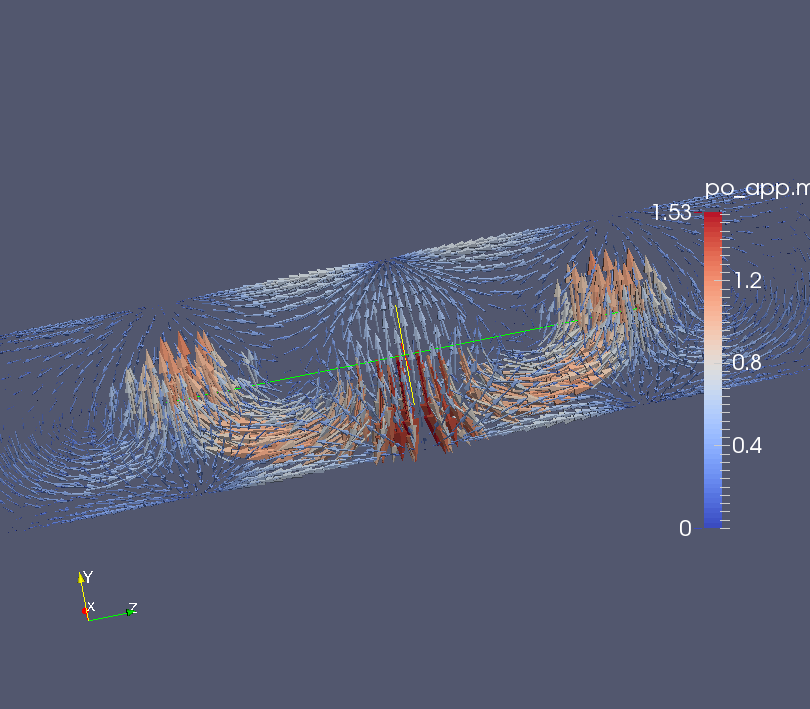
\includegraphics[scale=0.3]{curl-grad-1e3-mode0}}\ 
		\subfloat[mode 20]{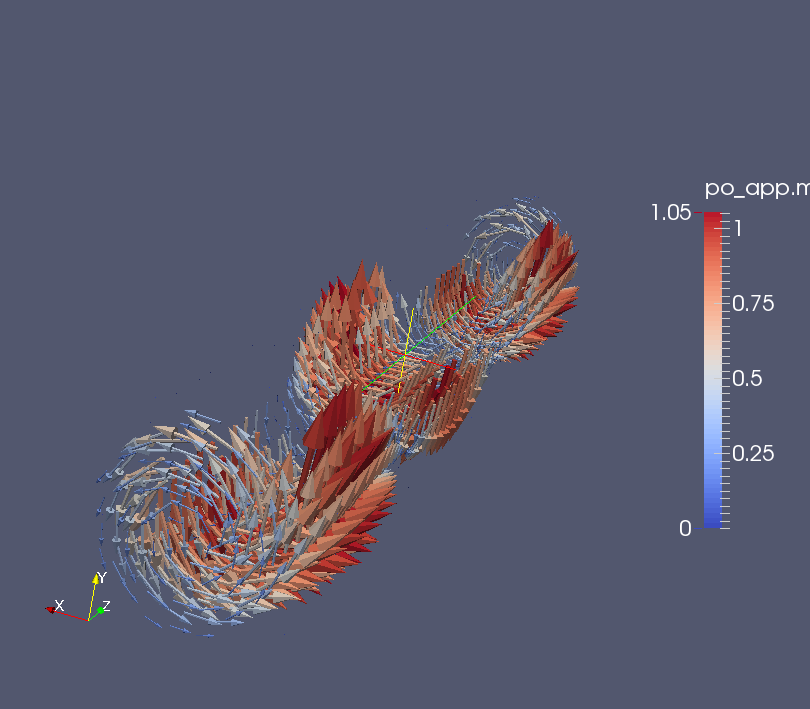
\includegraphics[scale=0.3]{curl-grad-1e3-mode20}}
	}\\
	\makebox[\textwidth][c]{
		\subfloat[mode 30]{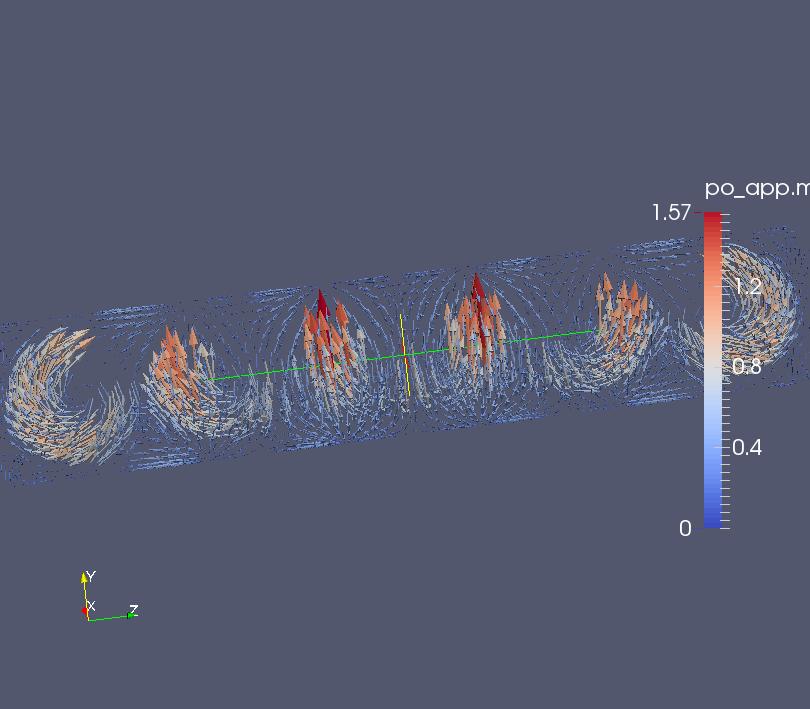
\includegraphics[scale=0.3]{curl-grad-1e3-mode30}}\ 
		\subfloat[mode 45]{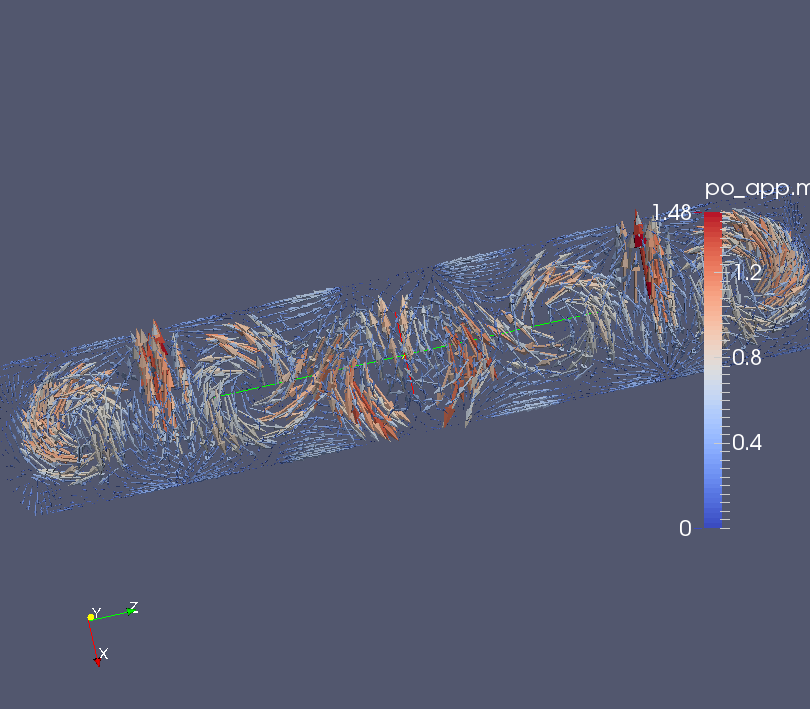
\includegraphics[scale=0.3]{curl-grad-1e3-mode45}}
	}
	\caption{Modes propres}
	\label{resultats}
\end{figure}

Cependant, dû au manque de puissance de ma machine de travail, je ne peux travailler sur un nombre élevé de maille, ce qui induit un manque de précision dans les calculs, et donc une faible régularité des fonctions calculées. L'opérateur rotationnel induit donc des erreurs. Ainsi, si on calcul l'erreur entre le rotationnel du champ et le champ multiplier par sa valeur propre, ou même lors du calcul de la condition $\rot\mathbf{g_i}\cdot\mathbf{n}$, nous n'obtenons pas les résultats escomptés :
\begin{center}
\begin{tabular}{ >{$}c<{$} | >{$}c<{$} | >{$}c<{$} | >{$}c<{$} | >{$}c<{$} | >{$}c<{$} | >{$}c<{$} | >{$}c<{$} | >{$}c<{$} }
\no & \lambda^2 & \lambda & \div\star & \star\cdot\mathbf{n} & \rot\star\cdot\mathbf{n} & ||\rot\star-\star|| & ||\star|| & ||\rot\star|| \\ \hline
10 & 49.1504 & 7.0107 & 0.00217561 & 0.0250946 & 0.208425 & 9.62716 & 0.999049 & 6.94417
\end{tabular}
\end{center}

De plus, en regardant les deux champs, on voit qu'ils n'ont pas la même forme. Par exemple, la figure \ref{eigendiff} montre la différence entre le 10\ieme\ vecteur propre et son rotationnel :

\begin{figure}[H]
	\makebox[\textwidth][c]{
		\subfloat[mode 10]{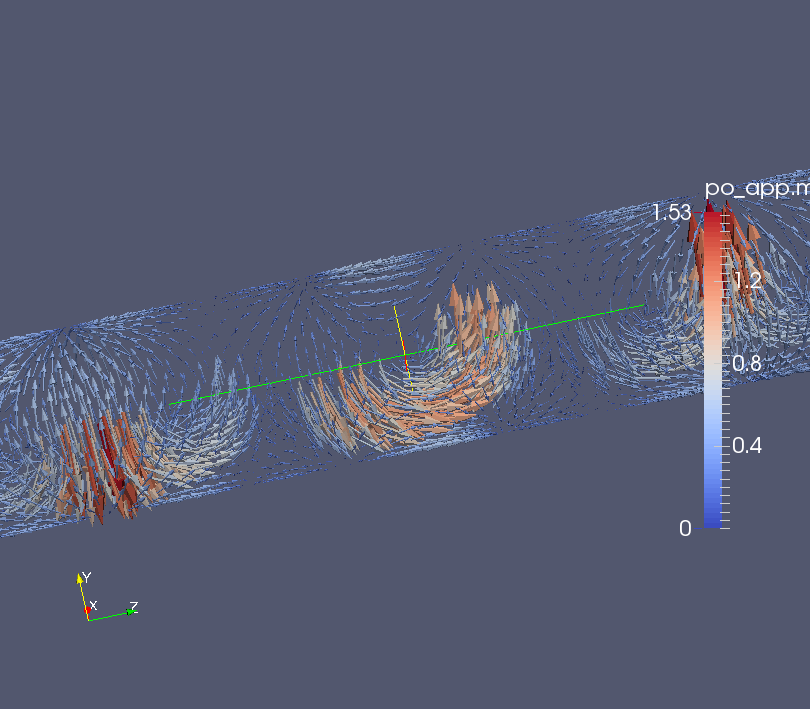
\includegraphics[scale=0.3]{mode10}}\ 
		\subfloat[$\rot($mode 10$)$]{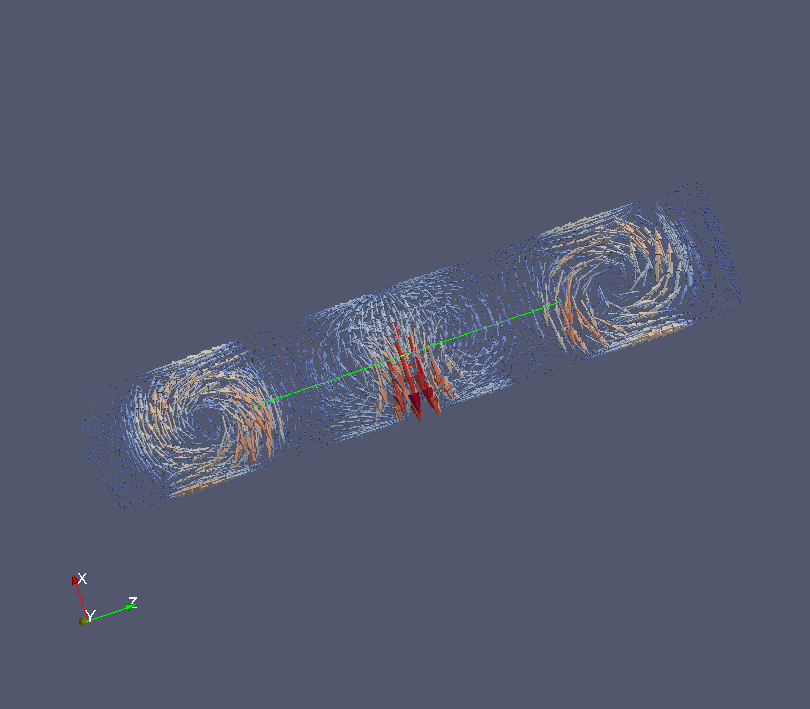
\includegraphics[scale=0.3]{curl10}}
	}
	\caption{Différences entre les modes et leur rotationnel}
	\label{eigendiff}
\end{figure}
Ces erreurs empêchent la vérification des résultats mais comme tous les calculs sur le rotationnel des modes propres sont remplacés par des calculs sur les fonctions propres multipliées par leur valeur propre respective, cela n'empêche pas la suite de la résolution du problème.\\

%% Cela peut aussi être dû aux paramètres de pénalisation, en effet si on change ces paramètres, on trouve des valeurs propres complètement différentes :

%% \begin{center}
%% \begin{tabular}{ >{$}c<{$} | >{$}c<{$} | >{$}c<{$} | >{$}c<{$} | >{$}c<{$} | >{$}c<{$} | >{$}c<{$} }
%% \alpha & \beta & \gamma & \lambda^2 & \div\star & \star\cdot\mathbf{n} & \rot\star\cdot\mathbf{n} \\ \hline
%% 0 & 0 & 0 & 5.24707e-11 & 15.0503 & 0.477078 & 1.23413e-07 \\ \hline
%% 10^3 & 10^3 & 10^3 & 40.9302 & 0.00210937 & 0.0232026 & 0.185115 \\ \hline
%% 10^6 & 10^6 & 10^6 & 57.1154 & 0.000159613 & 0.000673913 & 0.466915 \\ \hline
%% 10^{10} & 10^{10} & 10^{10} & 61.731 & 1.3273e-06 & 6.06696e-06 & 0.847356 \\ \hline
%% 10^{15} & 10^{15} & 10^{15} & 1.36827 & 2.30829e-09 & 5.37688e-08 & 5.57285 \\ \hline
%% 10^{10} & 10^3 & 10^3 & 42.0751 & 6.2461e-09 & 0.0310199 & 0.299304 \\ \hline
%% 10^3 & 10^{10} & 10^3 & 42.0096 & 0.00280563 & 0.0302683 & 0.280824 \\ \hline
%% 10^3 & 10^3 & 10^{10} & 57.5605 & 0.00622557 & 1.23812e-06 & 0.621214
%% \end{tabular}
%% \end{center}

%% Il y a donc un problème dans la méthode de pénalisation. Une explication pourrait être que les différents termes de pénalisation sont largement supérieurs aux termes correspondant au problème aux valeurs propres, et donc on ne résoudrait plus ce problème, mais un problème où la majorité des informations serait contenues dans les termes de pénalisation.\\

\subsection{Temps de calculs}
Les tests on été effectués sur une machine virtuelle Linux Debian 6, invitée sur un ordinateur avec 4 processeurs Intel Xeon cadencés à 2,4 GHz et 64 Go de RAM, mais avec seulement 47 Go de RAM alloués à la machine virtuelle.\\

J'ai effectué les tests sur les maillages suivants avec des éléments de Lagrange d'ordre 2 vectoriel pour $\mathbf{g}$ et d'ordre 1 scalaire pour $p$. \\

\begin{center}
\begin{tabular}{c|c|c|c|c|c}
h & éléments & DDL & DDL/2 & DDL/3 & DDL/4\\ \hline
0,15 & 5000 & 25000 & 12500 & 8500 & 6250\\ \hline
0.125 & 7500 & 40000 & 20000 & 13500 & 10000\\ \hline
0.1 & 12500 & 65000 & 32500 & 22000 & 16250
\end{tabular}
\end{center}

La figure \ref{timeM} montre les temps de calculs en fonction du nombre de modes propres, entre 1 et 150, pour différentes tailles de maillage et différents nombres de processeurs.\\

\begin{figure}[H]
\centering
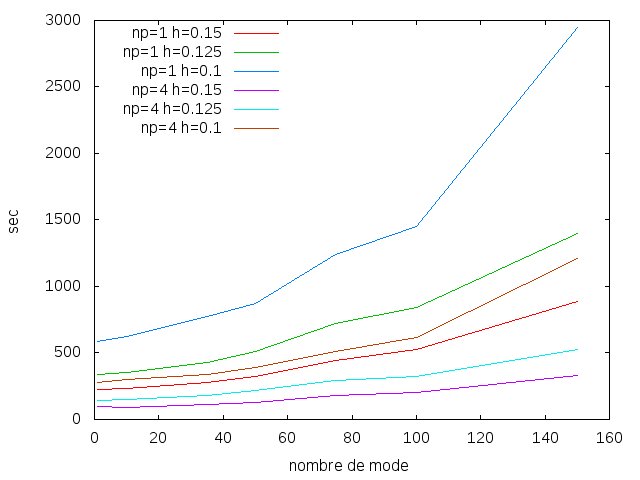
\includegraphics[scale=0.8]{timeM}
\caption{Temps de calcul en fonction du nombre de modes propres}
\label{timeM}
\end{figure}
Comme on s'y attend, le temps de calcul augmente en fonction du modes calculés. On voit que plus la taille de maillage est faible, plus le temps de calcul augmente rapidement. Toutefois, l'exécution en parallèle permet de réduire cette augmentation, comme le montre la figure \ref{timeNP}.
\begin{figure}[H]
\centering
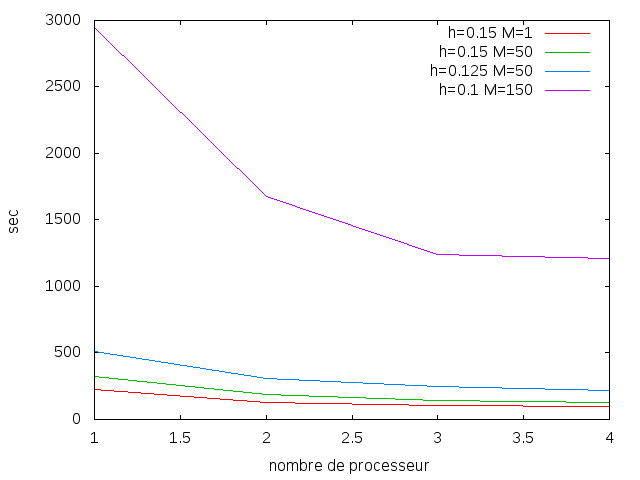
\includegraphics[scale=0.8]{timeNP}
\caption{Temps de calcul en fonction du nombre de processeurs}
\label{timeNP}
\end{figure}
On peut voir un net gain de temps entre l'exécution en séquentiel et en parallèle avec juste 2 processeurs. Même si en augmentant le nombre de processeurs on continue de diminuer le temps de calcul, le gain n'est plus aussi significatif, au fur et à mesure que la communication entre les processeurs augmente, alors que le temps de résolution des systèmes ne change pas.\\

On présente dans la figure \ref{timeH} le temps de calcul en fonction de la taille du maillage. Ces tests sont effectués avec 4 processeurs, pour 50 modes et des fonctions d'ordre 2 et 3 sur les maillages suivants :
\begin{center}
\begin{tabular}{c|c|c|c}
h & éléments & DDL Ordre 2 & DDL  Ordre 3\\ \hline
0.2 & 2000 & 11500 & 35000 \\ \hline
0.175 & 3000 & 17500 & 50000 \\ \hline
0,15 & 5000 & 25000 & 80000 \\ \hline
0.125 & 7500 & 40000 & 120000 \\ \hline
0.1 & 12500 & 65000 & 200000 \\ \hline
0.75 & 26500 & 135000 & 400000
\end{tabular}
\end{center}

\begin{figure}[H]
\centering
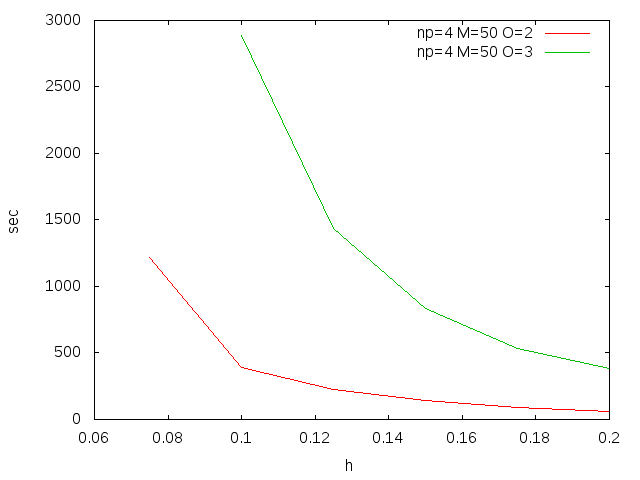
\includegraphics[scale=0.8]{timeH}
\caption{Temps de calcul en fonction de la taille de maillage}
\label{timeH}
\end{figure}

Comme on le voit, le temps de calcul augmente exponentiellement, ce qui a même empêché d'arriver au bout du calcul pour $h=0.1$ en ordre 3. Cependant, comme vu plus haut, plus le nombre de degré de liberté augmente, plus l'utilisation d'un grand nombre de processeurs est utile. On peut donc espérer qu'avec un nombre de processeurs bien supérieur, on puisse résoudre des problèmes de manière précise. 

% \section{Composante $z$}
% \subsection{Implémentation}
% \subsection{Résultats}

%%% Local Variables:
%%% TeX-master: "../report.tex"
%%% eval: (flyspell-mode 1)
%%% ispell-local-dictionary: "french"
%%% End:


\chapter{Relèvement}
\todo[inline]{intro ch + $\bm{e}$ ?? }
Dans le cas du cylindre, on a $\alpha_1=0$, ce qui conduit à ce que $\rot \mathbf{b}=0$ et donc $\mathbf{a}=\grad\psi^0$.

\section{Gradient dans $\HH^1$}
\label{impGradh1}
\subsection{Implémentation}
Si l'on veut utiliser le problème (\ref{pbpsi0}) dans $\HH^1$, alors il faut utiliser un multiplicateur de Lagrange pour ajouter une contrainte sur $\psi^0$, par exemple $\int \psi^0 = 0$. Cela se traduit par le changement de formulation variationnelle suivant où l'on cherche $(\psi^0,\lambda)\in \HH^1\times\R$ et où $(\varphi,\nu)$ est la fonction de test :
\[ \int_\Omega\grad \psi^0\grad\varphi + \int_\Omega \psi^0\nu + \int_\Omega \lambda\varphi = \int_{\partial\Omega} \alpha_0\varphi \]
On va donc créé un espace de fonction produit correspondant à $\HH^1\times\R$.

\lstinputlisting[linerange={space}]{../../src/psi0.hpp}

On ajoute une fonction permettant de rajouter en option le profil d'entrée en fonction du rayon et de la vitesse. Cela correspond à $\alpha_0$.

\lstinputlisting[linerange={option}]{../../src/psi0.cpp}

Une fois les éléments de l'espace créé, on peut définir la forme bilinéaire de la façon suivante :

\lstinputlisting[linerange={bilinear}]{../../src/psi0.cpp}

Ici, $u$ correspond à $\psi^0$ et $v$ à $\varphi$ et \texttt{inner} est le produit scalaire.\\

On veut que ce qui rentre du cylindre par l'entrée, correspondant à la partie du maillage marquée 1, sorte par l'autre bout du cylindre, marqué 2, et que le tour du cylindre, marqué 3, soit imperméable. Ce qui donne la terme de droite suivant :

\lstinputlisting[linerange={rhs}]{../../src/psi0.cpp}

Une fois le problème résolut, on veut projeter le gradient de $\psi^0$ sur $\LL^2$. Pour cela on résout le problème simple $u=\grad\psi^0$ qui mène à la forme variationnelle suivante :
\[ \int_\Omega \bm{u}\cdot\bm{v} = \int_\Omega \grad\psi^0\cdot\bm{v} \]

\lstinputlisting[linerange={gradpsi0}]{../../src/psi0.cpp}

\subsection{Résultats}
Dans les figure \ref{az},\ref{aIn},\ref{aOut}, on peut observer $\bm{a}$ dans le cylindre. Ici, $\alpha_1=0$ et 
\[ \alpha_0(x,y)= \begin{cases} -2\times v\times\left(1-\frac{x^2+y^2}{r^2}\right) &\mbox{sur } \Gamma_1\\
2\times v\times\left(1-\frac{x^2+y^2}{r^2}\right)&\mbox{sur } \Gamma_2\\
0 &\mbox{sur } \Gamma_3 \end{cases} \]

\begin{figure}[H]
\centering
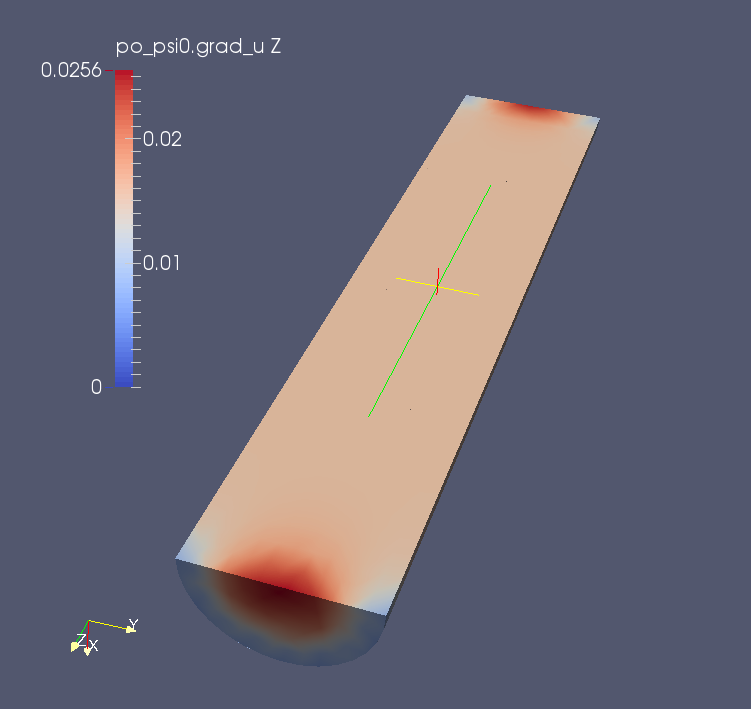
\includegraphics[scale=0.35]{az}
\caption{composante $z$ de $\bm{a}$}
\label{az}
\end{figure}
\begin{figure}[H]
\centering
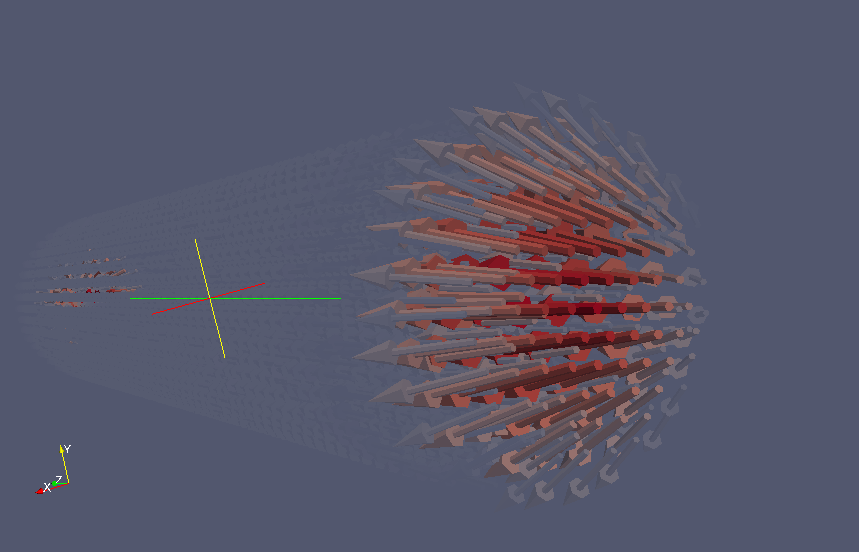
\includegraphics[scale=0.5]{aIn}
\caption{entrée du cylindre}
\label{aIn}
\end{figure}
\begin{figure}[H]
\centering
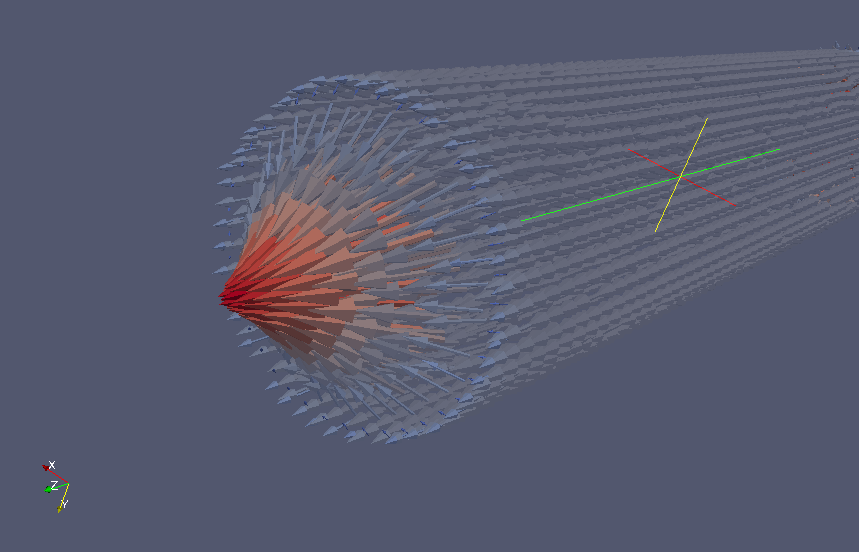
\includegraphics[scale=0.5]{aOut}
\caption{sortie du cylindre}
\label{aOut}
\end{figure}

%\section{Gradient dans $\HH(div)$}

%%% Local Variables:
%%% TeX-master: "../report.tex"
%%% eval: (flyspell-mode 1)
%%% ispell-local-dictionary: "french"
%%% End:


\section{Problème spectral}
\label{spectre}
Nous connaissons maintenant $\mathbf{a}$ et les couples $(\lambda_i,\mathbf{g}_i)_{i=1,\dots,M}$, on a donc toutes les briques pour trouver les coefficients $c_i$ de $\mathbf{u}_M$ l'approximation de $\mathbf{u}$ :
\[\mathbf{u}_M= \sum_{i=1}^M c_i\mathbf{g}_i\mbox{ tel que } \mathbf{u}_M\underset{M\rightarrow\infty}{\longrightarrow} \mathbf{u}=\sum_{i=1}^\infty c_i\mathbf{g}_i\]
Pour cela, on utilise l'approximation du problème \ref{pbc}.
\begin{align*}
\sum_{i=1}^M\frac{\partial c_i}{\partial t}\mathbf{g}_i &+ \sum_{i=1}^M\sum_{j=1}^Mc_ic_j(\curl\mathbf{g}_i\times \mathbf{g_j}) + \sum_{i=1}^Mc_i(\curl\mathbf{g}_i\times \mathbf{a})\\
& +  \sum_{i=1}^Mc_i((\curl\mathbf{a})\times \mathbf{g}_i) + \grad \pi_{\mathbf{a}} +\frac{1}{Re}\sum_{i=1}^Mc_i\curll\mathbf{g}_i - \mathbf{f_a} = 0\\
\end{align*}

Pour obtenir la forme variationnel du problème, on multiplie par une fonction test $\bm{\varphi}\in D^1(\Omega)$ et on intègre :
\begin{align*}
\sum_{i=1}^M\frac{\partial c_i}{\partial t}\int_\Omega\mathbf{g}_i\cdot\bm{\varphi} &+ \sum_{i=1}^M\sum_{j=1}^Mc_ic_j\int_\Omega(\curl\mathbf{g}_i\times \mathbf{g_j})\cdot\bm{\varphi} + \sum_{i=1}^Mc_i\int_\Omega(\curl\mathbf{g}_i\times \mathbf{a})\cdot\bm{\varphi}\\
& +  \sum_{i=1}^Mc_i\int_\Omega((\curl\mathbf{a})\times \mathbf{g}_i)\cdot\bm{\varphi} + \int_\Omega\grad \pi_{\mathbf{a}}\cdot\bm{\varphi} +\frac{1}{Re}\sum_{i=1}^Mc_i\int_\Omega\curll\mathbf{g}_i\cdot\bm{\varphi} - \int_\Omega\mathbf{f_a}\cdot\bm{\varphi} = 0\\
\end{align*}

En utilisant une intégration par partie sur le terme contenant $\grad\pi_{\mathbf{a}}$, on arrive à :
\begin{align*}
\sum_{i=1}^M\frac{\partial c_i}{\partial t}\int_\Omega\mathbf{g}_i\cdot\bm{\varphi} &+ \sum_{i=1}^M\sum_{j=1}^Mc_ic_j\int_\Omega(\curl\mathbf{g}_i\times \mathbf{g_j})\cdot\bm{\varphi} + \sum_{i=1}^Mc_i\int_\Omega(\curl\mathbf{g}_i\times \mathbf{a})\cdot\bm{\varphi}\\
& +  \sum_{i=1}^Mc_i\int_\Omega((\curl\mathbf{a})\times \mathbf{g}_i)\cdot\bm{\varphi} + \int_\Omega\pi_{\mathbf{a}}\div\bm{\varphi} + \int_{\partial\Omega}\pi_{\mathbf{a}}(\bm{\varphi}\cdot\mathbf{n})\\
& \frac{1}{Re}\sum_{i=1}^Mc_i\int_\Omega\curll\mathbf{g}_i\cdot\bm{\varphi} = \int_\Omega\mathbf{f_a}\cdot\bm{\varphi}\\
\end{align*}

\begin{rk}
Comme $\bm{\varphi}\in D^1(\Omega)$, $\div\bm{\varphi}=0$ et $\bm{\varphi}\cdot \mathbf{n}=0$ sur $\partial\Omega$, le terme de pression s'annule donc sous cette forme. Il sera recalculé en post-traitement, voir \ref{pression}.\\
\end{rk}
Ce qui donne :
\begin{align*}
\sum_{i=1}^M\frac{\partial c_i}{\partial t}\int_\Omega\mathbf{g}_i\cdot\bm{\varphi} &+ \sum_{i=1}^M\sum_{j=1}^Mc_ic_j\int_\Omega(\curl\mathbf{g}_i\times \mathbf{g_j})\cdot\bm{\varphi} + \sum_{i=1}^Mc_i\int_\Omega(\curl\mathbf{g}_i\times \mathbf{a})\cdot\bm{\varphi}\\
& +  \sum_{i=1}^Mc_i\int_\Omega((\curl\mathbf{a})\times \mathbf{g}_i)\cdot\bm{\varphi} + \int_\Omega\pi_{\mathbf{a}}\div\bm{\varphi} + \textcolor{red}{\frac{1}{Re}\sum_{i=1}^Mc_i\int_\Omega\curll\mathbf{g}_i\cdot\bm{\varphi}}\\
& = \int_\Omega\mathbf{f_a}\cdot\bm{\varphi}\\
\end{align*}

Le terme $\sum_{i=1}^Mc_i\int_\Omega\curll\mathbf{g}_i\cdot\bm{\varphi}$ provient de $\int_\Omega \curll\mathbf{u}\cdot\bm{\varphi}$.\\
En utilisant plusieurs intégrations par parties et la décomposition de $\bm{\varphi}$ dans $D^1(\Omega)$, cela devient $\int_\Omega\curl\mathbf{u}\cdot\curl\bm{\varphi} -\int_{\partial\Omega} \alpha_2\phi$.\\
En repassant à la décomposition de Galerkin, on obtient donc le terme $\sum_{i=1}^Mc_i\lambda_i\int_\Omega\mathbf{g}_i\cdot\curl\bm{\varphi}-\int_{\partial\Omega} \alpha_2\phi$.\\
\begin{rk}
  Cependant, on a que $\alpha_2=\curll\mathbf{u}\cdot\mathbf{n}\restr{\Gamma}=\sum c_i\lambda_i^2 \mathbf{g}_i\cdot\mathbf{n}\restr{\Gamma} = 0$.\\
Si l'on veut que cette condition soit différente de 0, $\alpha_2$ devrait être relever de la même manière que $\alpha_0$ et $\alpha_1$, mais comme cela a été remarqué tardivement, on a fait le choix de continuer à résoudre le système de la manière décrite dans ce rapport.\\
Pareillement, $\mathbf{b}$ appartient aussi à $D^1$, on ne devrait donc pas avoir $\curll\mathbf{b}\cdot\mathbf{n}\restr{\Gamma}=\alpha_1$.
\end{rk}
Lorsqu'on prend une fonction de test dans $D^1$, on cherche à ce que l'équation soit vrai pour toutes les fonctions de $D^1$. Cela revient au même que de résoudre cette équation pour toutes les fonctions de la base de $D^1$. On utilise donc encore une fois les fonctions propres de l'opérateur rotationnel.\\
On cherche donc $\forall k=1,\dots,M$ :
\begin{align*}
\sum_{i=1}^M\frac{\partial c_i}{\partial t}\int_\Omega\mathbf{g}_i\cdot\mathbf{g_k} &+ \sum_{i=1}^M\sum_{j=1}^Mc_ic_j\int_\Omega(\curl\mathbf{g}_i\times \mathbf{g_j})\cdot\mathbf{g_k} + \sum_{i=1}^Mc_i\int_\Omega(\curl\mathbf{g}_i\times \mathbf{a})\cdot\mathbf{g_k}\\
& +  \sum_{i=1}^Mc_i\int_\Omega((\curl\mathbf{a})\times \mathbf{g}_i)\cdot\mathbf{g_k} +\frac{1}{Re}\sum_{i=1}^Mc_i\lambda_i^2\int_\Omega\mathbf{g}_i\cdot\mathbf{g_k}-\frac{1}{Re}\int_{\partial\Omega} \alpha_2\phi_k = \int_\Omega\mathbf{f_a}\cdot\mathbf{g_k}\\
\end{align*}
Comme la base $(\mathbf{g}_i)$ est orthonormale, on a $\forall k=1,\dots,M$ :
\begin{align*}
\frac{\partial c_k}{\partial t} &+ \frac{1}{Re}c_k\lambda_k^2 + \sum_{i=1}^M\sum_{j=1}^Mc_ic_j\int_\Omega(\curl\mathbf{g}_i\times \mathbf{g_j})\cdot\mathbf{g_k}\\
& + \sum_{i=1}^Mc_i\int_\Omega(\curl\mathbf{g}_i\times \mathbf{a})\cdot\mathbf{g_k} +  \sum_{i=1}^Mc_i\int_\Omega((\curl\mathbf{a})\times \mathbf{g}_i)\cdot\mathbf{g_k} = \int_\Omega\mathbf{f_a}\cdot\mathbf{g_k}+\frac{1}{Re}\int_{\partial\Omega} \alpha_2\phi_k\\
\end{align*}
En utilisant les notations suivantes :
\begin{align*}
  R_{ijk} &= \int_\Omega(\curl\mathbf{g}_i\times \mathbf{g_j})\cdot\mathbf{g_k} & R_{iak} &= \int_\Omega(\curl\mathbf{g}_i\times \mathbf{a})\cdot\mathbf{g_k}\\
  &= \lambda_i\int_\Omega(\curl\mathbf{g}_i\times \mathbf{g_j})\cdot\mathbf{g_k} & &= \lambda_i\int_\Omega(\curl\mathbf{g}_i\times \mathbf{a})\cdot\mathbf{g_k}\\
R_{raij} &= \int_\Omega((\curl\mathbf{a})\times \mathbf{g}_i)\cdot\mathbf{g_k} & R_{hk} &= \int_\Omega\mathbf{f_a}\cdot\mathbf{g_k}\\
R_{pk} &= \int_{\partial\Omega} \alpha_2\phi_k
\end{align*}
Le problème \ref{pbc} devient :
\begin{pb}\label{fvc}
Trouver $(c_i)_{i=1,\dots,M}$ tel que $\forall k=1,\dots,M$ :
\begin{equation*}
\frac{\partial c_k}{\partial t} + \frac{1}{Re}c_k\lambda_k^2 + \sum_{i=1}^M\sum_{j=1}^Mc_ic_jR_{ijk} + \sum_{i=1}^Mc_iR_{iak} + \sum_{i=1}^Mc_iR_{raij} = R_{hk} + \frac{1}{Re}R_{pk}
\end{equation*}\end{pb}

\begin{rk}
$R_{ijk}$ et $R_{pk}$ ne sont à calculer qu'une seule fois. Si $\mathbf{a}$ dépend du temps, alors, les autres termes doivent être recalculés à chaque itération en temps.
\end{rk}
\begin{rk}
On a autant d'équations à résoudre et d'inconnus que de fonctions propres, c'est-à-dire $M$. Afin d'avoir une bonne approximation, on a besoin du plus grand nombre de fonctions de bases possible. Il faut donc trouver $M$ pour avoir un bon ratio entre précision et temps de calcul.
\end{rk}

%%% Local Variables:
%%% TeX-master: "../report.tex"
%%% eval: (flyspell-mode 1)
%%% ispell-local-dictionary: "french"
%%% End:


\section{Pression : Post-traitement de la vitesse}
\label{pression}
Pour retrouver la vitesse $\mathbf{v}$, il suffit maintenant d'additionner $\mathbf{a}$ et $\mathbf{u}$.\\
Le terme correspondant à la pression ayant été relayé en post-traitement de la vitesse, il faut le recalculer à partir de l'équation du problème \ref{depart}.

On applique la divergence sur cette équation et on utilise le fait que $\mathbf{v}$ soit à divergence nulle, et que la divergence d'un rotationnel soit toujours nulle. On a alors :
\begin{equation*}
-\laplace q = \div((\curl \mathbf{v})\times \mathbf{v}) - \div \mathbf{f}
\end{equation*}

Pour obtenir une condition au bord, on utilise la composante normale de l'équation (\ref{depart}) et les conditions aux bords de $\mathbf{v}$ :
\[ \grad q\cdot \mathbf{n}\restr{\Gamma} =  \mathbf{f}\cdot \mathbf{n}\restr{\Gamma} - \frac{\partial\alpha_0}{\partial t} - ((\curl \mathbf{v})\times \mathbf{v})\cdot \mathbf{n}\restr{\Gamma} - \frac{\alpha_2}{Re} \]
On cherche maintenant la forme variationnelle du problème :
\[ \int_\Omega -\laplace q\varphi = \int_\Omega (\div((\curl \mathbf{v})\times \mathbf{v}) -\div \mathbf{f})\varphi \]
En intégrant par partie le terme de gauche, on a :
\[ \int_\Omega \grad q\grad\varphi - \int_{\partial\Omega} (\grad q\cdot \mathbf{n})\varphi = \int_\Omega (\div((\curl \mathbf{v})\times \mathbf{v}) -\div \mathbf{f})\varphi \]

Toujours de même manière, on va trouver la pression à une constante près, on utilise donc encore une fois les multiplicateur de Lagrange afin de fixer cette constante. Comme dans \ref{multLagrange}, on obtient donc au final :
\begin{pb}\label{fvq}
Trouver $p=q-\frac{\mathbf{v}\cdot\mathbf{v}}{2} \in L^2(\Omega)$ tel que $\forall \varphi\in L^2(\Omega)$, on a :
\begin{align*}
\int_\Omega \grad q\grad\varphi + \int_\Omega \lambda\varphi + \int_\Omega q\nu &= \int_\Omega (\div((\curl \mathbf{v})\times \mathbf{v}) -\div \mathbf{f})\varphi\\
&+ \int_{\partial\Omega} \left(f\cdot \mathbf{n} - \frac{\partial\alpha_0}{\partial t} - ((\curl \mathbf{v})\times \mathbf{v})\cdot \mathbf{n} - \frac{\alpha_2}{Re}\right)\varphi
\end{align*}\end{pb}

%%% Local Variables:
%%% TeX-master: "../report.tex"
%%% eval: (flyspell-mode 1)
%%% ispell-local-dictionary: "french"
%%% End:


\chapter{Recapitulatif}

The steps to resolve the problm are :
\begin{enumerate}
\item compute the eigenpairs of the curl operator with problem \ref{pbweak},
  \todo[inline]{Ok}
\item decompose those functions with \ref{fvgi0} and \ref{fvpsiml},
  \todo[inline]{May be not necessary}
\item find $a_0$, using one of the following :
  \begin{itemize}
  \item solve \ref{fvpsi0} to have $a_0\in H^1$,
  \item solve \ref{fvpsidiv} to have $a_0\in H(\mathrm{div})$,
  \end{itemize}
  \todo[inline]{Ok}
\item solve \ref{fvbcurl} or \ref{pbbd1} to find $\curl\mbf{a}_1$,
  \todo[inline]{to check}
\item solve a system to determine to find $\mbf{a}_2$;
  \todo[inline]{to check}
\item recompose $\mbf{a}$ thanks to $\grad a_0$, $\curl\mbf{a}_1$ and $\mbf{a}_2$,
\item \label{itemsp} solve the spectral proble \ref{fvc} in order to find the coefficients $c_i$ for $i=0\dots M$,
  \todo[inline]{Ok}
\item rebuild $\mbf{u}=\sum c_i \mbf{g}_i$ and $\mbf{v}=\mbf{a}+\mbf{u}$,
\item compute the pressure in post-traitment with \ref{fvq}.
\end{enumerate}

We now have find our solution $(\mbf{v},p)$.\\
The first step depends only on the geometry, so we can reuse the eigen functions even after changing some parameters. The step \ref{itemsp} is the most time consumming one. We need to compute a lot of coefficient before starting. Luckily, the most of them depend only on the geometry, so we can compute them only once, but the others depend on the parameters and even worse, can also depend on the time, si we could have to recompute them at each time step.\\

The figure \ref{org3} graphically represents the problems to solve.\\

\begin{figure}
  \centering
  \begin{tikzpicture}[scale=\taille]
    \node[scale=\taille,text width=10cm] (ccyan) at (5,4) {{\color{cyan} Chemins pour $\psi^0\in H^1$}} ;
    \node[scale=\taille,text width=10cm] (cmagenta) at (5,3.5) {{\color{magenta} Chemins pour $\psi^0\in H(\mathrm{div})$}} ;
    \node[draw,scale=\taille,fill=green!50] (di) at (12,5) {Données initiales} ;
    \node[draw,scale=\taille,fill=blue!50] (si) at (12,4) {Solutions intermédiaires} ;
    \node[draw,scale=\taille,fill=yellow!50] (sim) at (12,3) {Sol. inter. dép. de la géométrie} ;
    \node[draw,scale=\taille,fill=red!50] (sf) at (12,2) {Solutions finales} ;

    \node[draw,scale=\taille,fill=green!50] (alpha0) at (0.75,2) {$\alpha_0$} ;
    \node[draw,scale=\taille,fill=LimeGreen,label={[xshift=-0.7cm](\ref{fvpsi0})}] (pba0) at (-0.5,-2){
      $\begin{aligned}
        -\laplace\psi^0&=0\\
        \grad\psi^0\cdot \mbf{n} &= \alpha_0
      \end{aligned}$
    } ;
    \node[draw,scale=\taille,fill=blue!50] (a0) at (-0.5,-3.5) {$a_0$} ;
    \node[draw,scale=\taille,fill=LimeGreen] (pbgrada0) at (-0.5,-4.75) {$w=\grad a_0$} ;
    \node[draw,scale=\taille,fill=LimeGreen,label={[xshift=0.8cm](\ref{fvpsidiv})}] (pba0div) at (2,-2){
      $\begin{aligned}
        \mbf{w}&=\grad a_0\\
        \div\mbf{w}&=0\\
        \mbf{w}\cdot \mbf{n} &= \alpha_0
      \end{aligned}$
    } ;
    \node[draw,scale=\taille,fill=blue!50] (grada0) at (0.75,-6.5) {$\grad a_0$} ;

    \node[draw,scale=\taille,fill=green!50] (alpha1) at (5,2) {$\alpha_1$} ;
    \node[draw,scale=\taille,fill=gray!50] (pba1) at (5,-2){
      $\begin{aligned}
        \curll \mbf{a}_1 &= \grad\psi^1\\
        \div \mbf{a}_1 &=0\\
        \mbf{a}_1\cdot \mbf{n} &= 0\\
        \curl \mbf{a}_1\cdot \mbf{n} &= 0\\
        \grad \psi^1\cdot \mbf{n} &= \alpha_1
      \end{aligned}$
    } ;
    \node[draw,scale=\taille,fill=blue!50] (a1) at (5,-6.5) {$\curl\mbf{a}_1$} ;

    \node[draw,scale=\taille,fill=green!50] (alpha2) at (8,2) {$\alpha_2$} ;
    \node[draw,scale=\taille,fill=gray!50] (pba2) at (8,-2){
      $\begin{aligned}
        \curll \mbf{a}_2 &= \bm{\epsilon}\\
        \div \mbf{a}_2 &=0\\
        \mbf{a}_2\cdot \mbf{n} &= 0\\
        \curl \mbf{a}_2\cdot \mbf{n} &= 0\\
        \bm{\epsilon}\cdot \mbf{n} &= \alpha_2
      \end{aligned}$
    } ;
    \node[draw,scale=\taille,fill=blue!50] (a2) at (8,-6.5) {$\mbf{a}_2$} ;

    \node[draw,scale=\taille,fill=gray!50,label={[xshift=-1.3cm](\ref{a})}] (pba) at (3,-9) {$\mbf{a} = \grad a_0 + \curl \mbf{a}_1 + \mbf{a}_2$} ;
    \node[draw,scale=\taillem,fill=blue!50] (a) at (3,-12) {$\mbf{a}$} ;

    \node[draw,scale=\taille,fill=LimeGreen,label={[xshift=1.0cm](\ref{pbcond})}] (pbcond) at (11.5,-2){
      $\begin{aligned}
        \curl \mbf{u} = \lambda \mbf{u} & \quad \mbox{in }\Omega\\
        \curl \mbf{u}\cdot\mbf{n} = 0 & \quad \mbox{on }\Gamma
      \end{aligned}$
    } ;
    \node[draw,scale=\taille,fill=yellow!50] (lambdagi) at (11.5,-6.5) {$(\lambda_i^2,\mbf{g}_i)$} ;

    \node[draw,scale=\taille,fill=green!50] (f) at (8,-9) {$f$} ;
    \node[draw,scale=\taille,fill=green!50] (c0) at (9,-9) {$c_k^0$} ;
    \node[draw,scale=\taille,fill=ProcessBlue,label={[xshift=3.2cm](\ref{fvc})}] (pbsp) at (9,-12){
      $\begin{aligned}
        \frac{\partial c_k}{\partial t} &+ \sum_i\sum_j c_i c_j(\curl\mbf{g}_i\times \mbf{g_j}, \mbf{g_k}) \\
        &+ \sum_i c_i(\curl\mbf{g}_i\times \mbf{a},\mbf{g_k}) + \sum_i c_i((\curl \mbf{a})\times \mbf{g}_i, \mbf{g_k}) \\
        &+ \frac{1}{Re}c_k\lambda_k^2 = (\mbf{f_a},\mbf{g_k})
      \end{aligned}$
    } ;
    \node[draw,scale=\taille,fill=blue!50] (ck) at (9,-15) {$c_k$} ;
    \node[draw,scale=\taille,fill=gray!50,label={[xshift=0.7cm](\ref{u})}] (pbu) at (9,-16) {$\mbf{u}=\sum c_kg_k$} ;
    \node[draw,scale=\taillem,fill=blue!50] (u) at (9,-17) {$\mbf{u}$} ;
    \node[draw,scale=\taille,fill=gray!50,label={[xshift=0.6cm](\ref{v})}] (pbv) at (3,-18) {$\mbf{v}=\mbf{a}+\mbf{u}$} ;
    \node[draw,scale=\tailleg,fill=red!50] (v) at (3,-19) {$\mbf{v}$} ;
    \node[draw,scale=\taille,fill=gray!50,label={[xshift=3.1cm](\ref{fvq})}] (pbq) at (9,-19){
      $\begin{aligned}
        -\laplace q = \div((\curl \mbf{v})\times \mbf{v}) - \div \mbf{f}\\
        \grad q\cdot \mbf{n}\restr{\Gamma} =  \mbf{f}\cdot \mbf{n}\restr{\Gamma} - \frac{\partial\alpha_0}{\partial t} - ((\curl \mbf{v})\times \mbf{v})\cdot \mbf{n}\restr{\Gamma} - \frac{\alpha_2}{Re}
      \end{aligned}$
    } ;
    \node[draw,scale=\tailleg,fill=red!50] (q) at(15,-19) {$p$} ;

    \draw[->,>=latex,cyan] (-1,4) -- (ccyan) ; \draw[->,>=latex,magenta] (-1,3.5) -- (cmagenta) ;
    \draw (alpha0) -- (0.75,0); \draw[->,>=latex] (grada0) -- (pba) ; \draw[->,>=latex,cyan] (0.75,0) -| (pba0) ; \draw[->,>=latex,cyan] (pba0) -- (a0) ; \draw[->,>=latex,cyan] (a0) -- (pbgrada0) ; \draw[->,>=latex,cyan] (pbgrada0) -- (grada0) ; \draw[->,>=latex,magenta] (0.75,0) -| (pba0div) ; \draw[->,>=latex,magenta] (pba0div) -- (grada0) ; \draw[->,>=latex] (grada0) -- (pba) ;
    \draw[->,>=latex] (alpha1) -- (pba1) ; \draw[->,>=latex] (pba1) -- (a1) ; \draw[->,>=latex] (a1) -- (pba) ;
    \draw[->,>=latex] (alpha2) -- (pba2) ; \draw[->,>=latex] (pba2) -- (a2) ; \draw[->,>=latex] (a2) -- (pba) ;
    \draw[->,>=latex] (pba) -- (a);
    \draw[->,>=latex] (pbcond) -- (lambdagi); \draw[->,>=latex] (lambdagi) -- (pbsp) ;
    \draw[->,>=latex] (a) -- (pbsp); \draw[->,>=latex] (f) -- (pbsp); \draw[->,>=latex] (c0) -- (pbsp);
    \draw[->,>=latex] (pbsp) -- (ck); \draw[->,>=latex] (ck) -- (pbu); \draw[->,>=latex] (pbu) -- (u); \draw[->,>=latex] (u) -- (pbv); \draw[->,>=latex] (a) -- (pbv); \draw[->,>=latex] (pbv) -- (v); \draw[->,>=latex] (v) -- (pbq); \draw[->,>=latex] (pbq) -- (q);
  \end{tikzpicture}
  \caption{Flow chart of the problems to solve}
  \label{org3}
\end{figure}

%%% Local Variables:
%%% TeX-master: "../report.tex"
%%% eval: (flyspell-mode 1)
%%% ispell-local-dictionary: "english"
%%% End:
